\section{Применение выпарных аппаратов при выпаривании фильтрата барды}

\subsection{Выпарные аппараты общего назначения}

% Промышленный выпарной аппарат \cite{Shinsuke.Industrial.2005} представлен на \cref{fig:industial_evaporation_app}.
% 
% \begin{wrapfigure}{R}{0.5\textwidth}
% \centering
% \includegraphics[width=0.48\textwidth]{figures/temp/shinsuke.jpg}
% \caption{Промышленный выпарной аппарат: 1 "--- патрубок исходной жидкости, 2 перфорированная пластина, 3 "--- зона подачи исходной жидкости, 4 "--- направляющие, 5 "--- зона испарения, 6 "--- патрубок удаления выпаренного раствора, 7 "--- патрубок удаления жидкости, 8 "--- насос удаления жидкости, 9 "--- патрубок
% подачи теплового агента, 10 "--- боковая стенка корпуса зоны испарения, 11 "--- конусная стенка зоны испарения, 20 "--- жидкость на выходе.}\label{fig:industial_evaporation_app}
% \end{wrapfigure}

% Выпарной аппарат с восходящей и нисходящей пленками \cite{Petrov.Vyparnoy.2002} изображен на~\cref{fig:evaporation_app_up_down} 
% 
% \begin{wrapfigure}{R}{0.5\textwidth}
% \centering
% \includegraphics[width=0.48\textwidth]{figures/temp/petrov.jpg}
% \caption{Выпарной аппарат с восходящей и нисходящей пленками}\label{fig:evaporation_app_up_down}
% \end{wrapfigure}
\begin{wrapfigure}{r}{0.5\textwidth}
\centering
\includegraphics[width=0.48\textwidth]{figures/temp/ostrikov.jpg}
\caption[Вакуум-выпарной аппарат]{Вакуум-выпарной аппарат: 1~"--- корпус, 2~"--- верхняя крышка, 5, 6~"--- патрубки для удаления испаряемых паров, 7~"--- рубашка, 8~"--- патрубок для подвода горячего теплоносителя, 9~"--- патрубок для отвода отработанного теплоносителя, 3~"--- комбинированная мешалка, скребки: 20, 22~"--- серповидные, 21~"--- лемехообразные, 26~"--- нижняя камера аппарата, 27~"--- верхняя камера аппарата, 12, 13~"--- трубопровод, 25~"--- сепаратор, 4, 19~"--- подшипниковые опоры, 23~"--- вал, 11~"--- форсунки, 14~"--- насос, 28~"--- торообразная камера, 15~"--- распылительные форсунки, 17~"--- торцевые уплотнения, 16~"--- электродвигатель, 29~"--- муфта, 6~"--- патрубок, 18~"--- полое кольцо, 10~"--- кольцевой желоб, 24~"--- патрубок удаления продукта.}\label{fig:evaporation_app_ostrikov}
\end{wrapfigure}
Вакуум-выпарной аппарат \cite{Ostrikov.Vakuum.2011} (рисунок~\ref{fig:evaporation_app_ostrikov}) работает следующим образом: включается привод вакуум-насоса (не показан), соединенного с патрубками 5 и 6, и в камерах 26 и 27 создается заданная величина разрежения.
Одновременно в рубашку 7 через патрубок 8 подается горячий теплоноситель с заданной температурой, нагревая внутреннюю боковую стенку в камерах 26 и 27.
Далее включается регулируемый привод (не показан), который приводит во вращательное движение мешалку 3.
Также включается электродвигатель 16, приводящий во вращательное движение форсунки 15.
Затем подогретое до заданной температуры исходное фруктовое или овощное пюре нагнетательным насосом (не показан) подается через трубу 12 во вращающиеся форсунки 11.
За счет конструкции распылительных форсунок 11 продукт (фруктовое или овощное пюре) распыливается в виде мелкодиспергированных капель, имеющих
колоколообразную форму.
Затем капли фруктового или овощного пюре оседали на поверхности конусной части корпуса 1, формируя пленку продукта, которая с помощью серповидных скребков 20, закрепленных на мешалке 3, перемещалась к выгрузочному отверстию, соединенному с трубопроводом 13.
Серповидные скребки 20 не только перемещают продукт к трубопроводу 13, но и интенсивно его перемешивают, обеспечивая при этом дополнительное выпаривание влаги из продукта, т.к. внутренняя поверхность камер 26 и 27 обогревается с помощью рубашки 7. 
При этом за счет дополнительного нагрева продукта от поверхности конусной части корпуса 1 происходит дополнительное выпаривание влаги из продукта.
Испаряемые из пюре водяные пары в нижней камере 26 удаляются через патрубок 6, соединенный с вакуум-насосом.
Далее продукт по трубопроводу 13 нагнетается насосом 14 в кольцевую торообразную камеру 28, на боковой поверхности которой с равным шагом радиально расположены распылительные форсунки 15.
Вращающиеся при помощи электродвигателя 16 и муфты 29 распылительные форсунки 15 распыливают продукт (фруктовое или овощное пюре) в виде мелкодиспергированных капель.
Форма и конструкции форсунок 15 обеспечивали равномерный режим распыливания по всему объему камеры 27. 
Затем капли фруктового или овощного пюре оседали на поверхности цилиндрической части корпуса 1, образуя пленку продукта, постепенно стекающую вниз под действием сил тяжести.
При контакте капель пюре с обогреваемой поверхностью происходил нагрев пленки пюре, стекающей вниз, и испарение влаги из пюре за счет термостатируемой внутренней стенки вакуум-выпарного аппарата.
Лемехообразные скребки 21, установленные на мешалке 3, счищают и постепенно плавно перемещают вниз слой овощного или фруктового пюре.
Серповидные скребки 22, установленные на мешалке 3, предназначены для удаления продукта с верхней поверхности сепаратора 25 и нанесения продукта тонким равномерным слоем по внутренней цилиндрической поверхности камеры 26.
Испаряемые из пюре водяные пары в верхней камере 27 удаляются через патрубки 5, соединенные с вакуум-насосом.
Концентрированный продукт (сгущенная суспензия), стекая по вертикальной
боковой стенке нижней камеры 26, попадает в кольцевой желоб 10 и выводится из аппарата через патрубок 24 для дальнейшей переработки.
\begin{figure}[htb]
\centering
\includegraphics[width=0.52\textwidth]{figures/temp/voynov.jpg}
\caption[Пленочный выпарной аппарат]{Пленочный выпарной аппарат: 1~"--- вертикальный цилиндрический корпус, 2~"--- крышка, 3~"--- днище, штуцера: 4,5~"---  для ввода и вывода раствора, 6~"--- вывода конденсата вторичного пара, 7, 8~"--- подвода и отвода теплоносителя, 9, 10~"--- подвода и отвода хладагента, 11~"--- вспомогательный, 12, 13~"--- камеры для ввода раствора и вывода концентрированного раствора, 14~"--- греющая камера, трубопроводы: 15, 16~"--- для подвода и отвода хладагента, 17~"--- отвода конденсата вторичного пара, 18~"--- цилиндрические трубы, 19~"--- кольцевая спираль, 20~"--- внутренние трубы, 21~"--- витки, 22~"--- патрубок для отвода конденсата вторичного пара, 23~"--- шайбы, 24~"--- ограничительные ребра, 25~"--- профилированные пластины, 26~"--- боковая кромка, 27~"--- каналы для прохода парожидкостной смеси, 28~"--- втулка для распределения жидкости, 29~"--- заглушка, 30~"--- ребра для обеспечения зазора и крепления, 31~"--- продольные канавки для отвода уловленных капель раствора, 32~"--- лист из пористого материала, 33~"--- воронки, 34~"--- пластинки, 35~"--- зазор для прохода конденсата вторичного пара.}\label{fig:evaporation_app_voynov}
\end{figure}

Пленочный выпарной аппарат \cite{Voynov.Plenochniy.2006} представлен на~\cref{fig:evaporation_app_voynov}.
Раствор через штуцер 4 поступает в камеру 12, распределяется на верхней горизонтальной перегородке, а затем поступает в кольцевые зазоры, образованные внутренней поверхностью цилиндрической трубы 18 и наружной поверхностью втулки, для распределения жидкости 28, выйдя из которых, раствор стекает в виде жидкостной пленки по внутренней поверхности цилиндрических труб, интенсивно перемешиваясь, обтекая витки кольцевой спирали 19.
При этом происходит нагревание раствора через стенку цилиндрических труб теплоносителем, поступающим через штуцер 7 в греющую камеру 14, вследствие чего раствор закипает, образуется отток вторичного пара и капель раствора (парожидкостная смесь) с поверхности пленки.
Парожидкостная смесь проходит по каналам 27, образованным профилированными пластинами 25, приобретает вращательнопоступательное движение, вследствие чего возникает центробежная сила, которая отбрасывает часть капель на поверхность пластин, которые затем по канавкам 31 стекают в камеру концентрированного раствора 13.
В случае наличия на поверхности пластин листа 32, выполненного из перфорированного материала, капли раствора по каналам, образованным порами пористого материала, также стекают вниз в камеру 13.
Другая часть капель в месте с потоком вторичного пара, выйдя из каналов 27, вследствие вращательного движения приобретает форму жидкостного кольца и под действием силы тяжести стекает вниз в камеру 13.
Освободившийся от капель вторичный пар конденсируется на поверхности внутренних труб 20, в полость которых подается охлаждающая вода через штуцер 9 и трубопроводы 15.
Отвод охлаждающей воды осуществля ется через трубу 16, соединенную со штуцером 10.
Образовавшийся конденсат по виткам 21 поступает на поверхность воронок 33 и через зазоры 35 стекает во внутрь витков, а затем в полость патрубков 22, через которые по трубопроводу 17 выводится из аппарата.
Сконцентрированный раствор на выходе из цилиндрических труб поступает в камеру 13, а затем через штуцер 5 выводится из аппарата.

\subsection{Барботажно-выпарные аппараты}
\begin{wrapfigure}{R}{0.52\textwidth}
\centering
\includegraphics[width=0.4\textwidth]{figures/temp/rabiner.jpg}
\caption[Выпарной аппарат для концентрирования растворов путем непосредственного контакта с газообразным теплоносителем]{Выпарной аппарат для концентрирования растворов путем непосредственного контакта с газообразным теплоносителем: 1~"--- вертикальный корпус, 2~"--- крышка, патрубки: 3~"--- подачи исходного раствора, 4~"--- отвода упаренного раствора, 5~"--- отвода парогазовой смеси, 6~"--- барботажные трубы, 7~"--- циркуляционная труба, 8~"--- кольцевой кожух, 9, 10~"--- коаксиальный цилиндр.}\label{fig:evaporation_app_rabiner}
\end{wrapfigure}
Выпарной аппарат (рисунок~\ref{fig:evaporation_app_rabiner}) для концентрирования растворов путем непосредственного контакта с газообразным теплоносителем~\cite{Rabiner.Vypanroy.1979} работает следующим образом: газообразный теплоноситель, например продукты сгорания топлива, по барботажным трубам 6 поступает в кольцевой кожух 8, откуда распределяется в центральную часть кожуха, ограниченную внутренним цилиндром 9, и в объем между циркуляционной трубой 7 и наружным цилиндром 10 кожуха 8.
Исходный раствор по патрубку 3 подается в центральную часть кожуха 8, где он в противотоке взаимодействует с газообразным теплоносителем, выходящим из полости кожуха 8.
Одновременно газообразный теплоноситель в объеме между циркуляционной трубой 7 и кожухом 8, двигаясь в прямотоке с раствором, создает его естественную циркуляцию в аппарате 1.
Упаренный раствор накапливается в нижней части аппарата 1 и непрерывно выводится через патрубок 4.
Парогазовая смесь сепарируется на жалюзийных насадках и непрерывно выводится из аппарата через патрубок 5.

\begin{figure}
\centering
\begin{minipage}{.45\textwidth}
\centering
\includegraphics[width=0.8\textwidth]{figures/temp/kasatkin.jpg}
\caption[Выпарной аппарат погружной горелкой]{Выпарной аппарат погружной горелкой:  1~"--- корпус, 2~"--- горелка, 3~"--- переливная труба, 4~"--- сепаратор.}\label{fig:evaporation_app_kasatkin}
\end{minipage}%
~
\begin{minipage}{.45\textwidth}
\centering
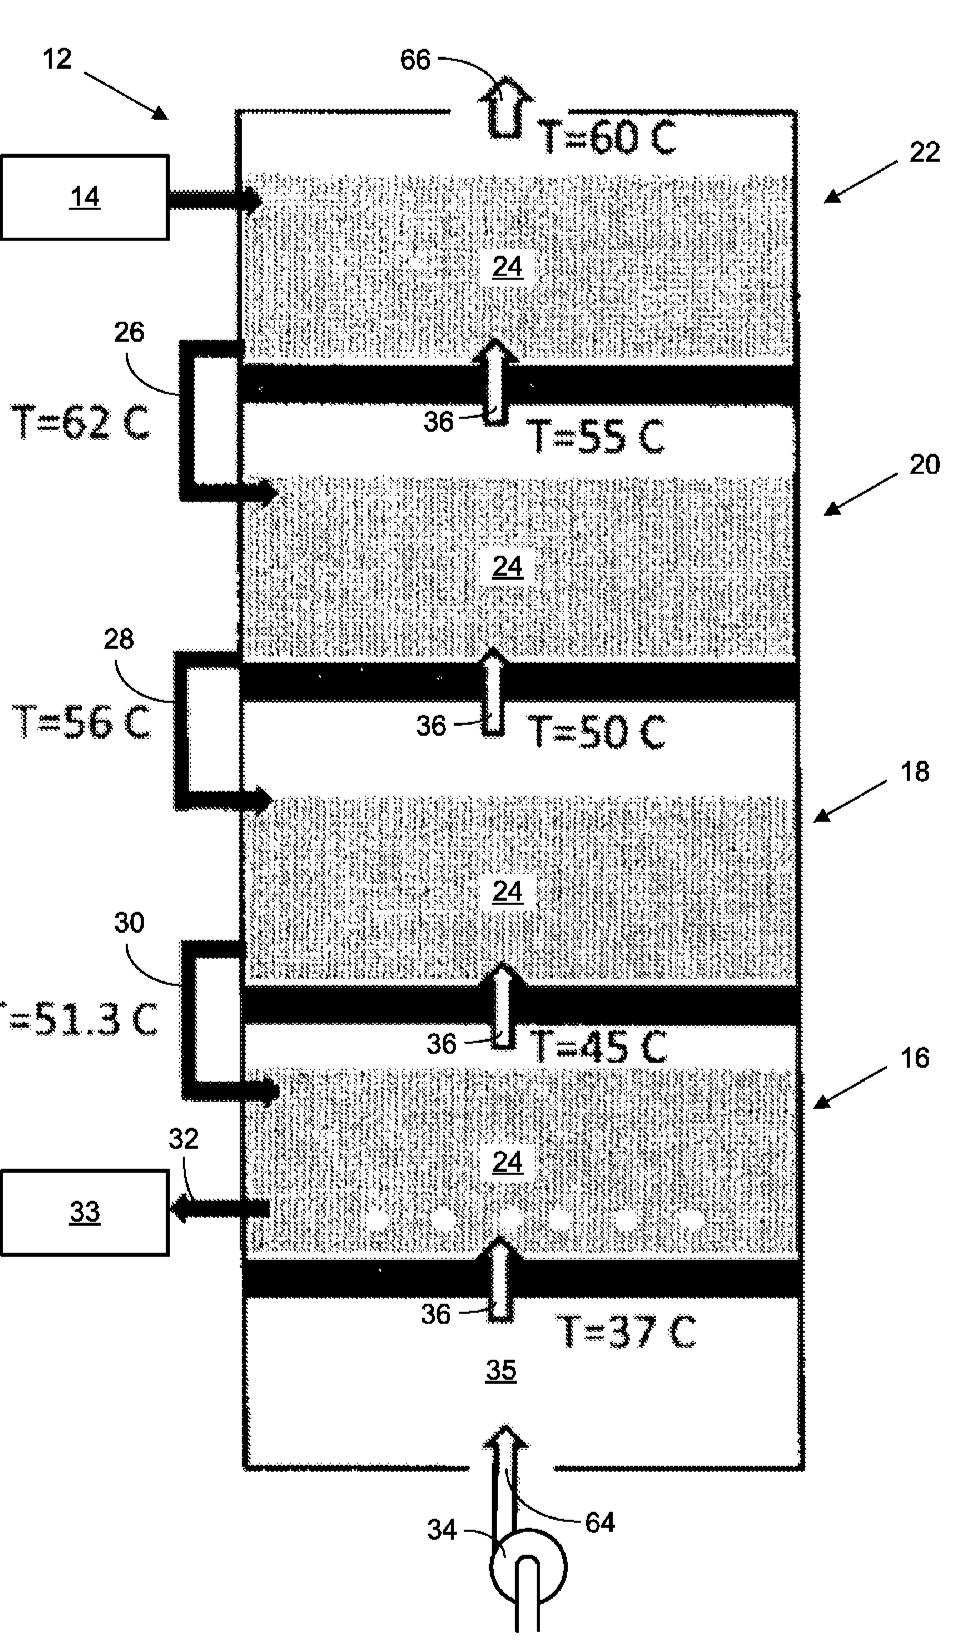
\includegraphics[width=0.5\textwidth]{figures/temp/Govindan.jpg}
\caption[Многокорпусной барботажно-выпарной аппарат]{Многокорпусной барботажно-выпарной аппарат: 12~"--- аппарат, 16, 18, 20, 22~"--- камера испарителя, 24~"--- ванна, 26, 28, 30, 32~"--- трубопровод, 34~"--- вентилятор, 64~"--- воздуховод.}\label{fig:evaporation_app_govindan}
\end{minipage}
\end{figure}


Барботажный выпарной аппарат с погружными горелками~\cite{Kasatkin.Processi.1971} изображен на~\cref{fig:evaporation_app_kasatkin}.
В плоской крышке корпуса 1 аппарата расположена одна горелка 2 или несколько горелок, погруженных под уровень выпариваемого раствора.
Уровень раствора в аппарате поддерживается постоянным с помощью переливной трубы 3.
Упаренный раствор отводится из конического днища аппарата, а выпадающие здесь кристаллы отсасываются посредством эрлифта.
Паро-газовая смесь от водится из пространства над жидкостью через сепаратор 4.
Многокорпусной барботажно-выпарной аппарат \cite{Govindan.Multi.2015} представлен на~\cref{fig:evaporation_app_govindan}.
Жидкость, содержащую растворенные компоненты подают из сборника 14 в камеру 22 испарителя 12, где жидкость образует ванну 24, содержащейся в камере четвертого стадии 22.
Исходную жидкость подают в камеру 22 для увлажнения четвертой стадии при температуре 70\(\celcius\).
Испаренный компонент (например, вода) из исходной жидкости испаряется газом, пузырьки которого подают через ванну 24.
Остатки жидкости подают из камеры 22 по трубопроводу 26 в камеру третьей ступени 20, в которой подают газ.
Остаток исходной жидкости подают в камеру третьей ступени 20 при температуре 62 С
Температура оставшейся жидкости уменьшается от стадии к стадии, в частности, с помощью энергии, используемой для испарения испаряемого компонента из исходной жидкости на каждой стадии.

Аппарат для перегонки улучшенной эффективности~\cite{Lee.Fluid.2007} представлен на~\cref{fig:evaporation_app_lee}.
Цилиндрический корпус 100 выполнен с возможностью контроля уровня воды или других жидкостей 111.
Воду или другие жидкости для дистилляции 112 подают в корпус 100 через впускное отверстие 113.
Сливной патрубок 114 предназначен для периодического удаления солоноватой жидкости конденсатора, который собирается в нижней части корпуса 100.
Паровое пространство 116 сформировано на верхнем конце внутренней корпуса 100, как правило над поверхностью жидкости 111.
Множество спиральных конденсирующих труб 117 расположены кольцеобразно на внешней периферии внутренней части корпуса 100.
Пар из парового пространства 116 поступает в конденсационные трубы 117, как указано стрелками 126 и 130.
Пары идущий по конденсационным трубам 117 вступает в теплообмен с жидкостью и конденсируется, производя дистиллят.
Дистиллят удаляют через коллектор 118 он содержит общее выпускное отверстие 119.
Барботирование газом 121 по трубе 122, имеющей отверстия 123 осуществляют в межтрубное пространство теплообменных труб 117, которые производят пузыри 124.
\begin{figure}[tb]
\centering
\includegraphics[width=0.5\textwidth]{figures/temp/lee.jpg}
\caption[Аппарат для перегонки улучшенной эффективности]{Аппарат для перегонки улучшенной эффективности: Цилиндрический корпус 100, уровень 111 жидкости, жидкости для дистилляции 112, впускное отверстие 113, сливной патрубок 114, паровое пространство 116, спиральные конденсирующие трубы 117, пар 126 и 130, коллектор 118, выпускное отверстие 119, камера конденсация 120, газ 121, труба для барботирования 122, отверстия для барботирования 123, пузыри 124, камера нагрева 127, трубчатая стенка 131, нагревательный элемент 128.}\label{fig:evaporation_app_lee}
\end{figure}
Пузыри поднимаются вверх в кольцевую камеру конденсации 120.
Геометрия камеры нагрева 127 задается трубчатой стенкой 131, окружающей нагревательный элемент 128.
Вода из камеры 120 конденсации проходит в глубь нагревательной камеры 127 через отверстие 133 в нижней ее части.
Нагревательный элемент 128 производит пузырьки пара 132, которые проходят вверх через верхнее отверстие 129 в камере нагрева в паровое пространство 116.
Затем пар поступает в конденсационные трубы, как показано стрелкой 130, и было описано ранее.


